% https://github.com/martinhelso/MathDept


\documentclass[UKenglish,8pt,aspectratio=1610]{beamer}

\usepackage[
backend=biber,        % compilateur par défaut pour biblatex
sorting=none,          % trier par nom, année, titre
citestyle=numeric, % style de citation auteur-année
bibstyle=numeric,  % style de bibliographie alphabétique
]{biblatex}
\addbibresource{biblio.bib}

\usetheme[NoLogo]{MathDept}
\usepackage{bbold}
\usepackage{nicematrix}
\usepackage{varwidth}
\usepackage[utf8]{inputenx} % For æ, ø, å
\usepackage{babel}          % Automatic translations
\usepackage{csquotes}       % Quotation marks
\usepackage{microtype}      % Improved typography
\usepackage{amssymb}        % Mathematical symbols
\usepackage{mathtools}      % Mathematical symbols
\usepackage[absolute, overlay]{textpos} % Arbitrary placement
\setlength{\TPHorizModule}{\paperwidth} % Textpos units
\setlength{\TPVertModule}{\paperheight} % Textpos units
\usepackage{tikz}
\usetikzlibrary{overlay-beamer-styles}  % Overlay effects for TikZ
\usepackage{dsfont}
\usepackage{fontawesome5}
\author{Thomas Aussaguès}
\title{Mandatory exercise 3}
\subtitle{MIMO Pulse-echo imaging}
\usepackage{siunitx}
\usepackage{graphics}
\graphicspath{{../images/}}	
\usepackage{pgfplots}
\DeclareUnicodeCharacter{2212}{−}
\usepgfplotslibrary{groupplots,dateplot}
\usetikzlibrary{patterns,shapes.arrows}
\pgfplotsset{compat=newest}
\usepackage{color}
\usepackage{colortbl}
\definecolor{darkred}{rgb}{0.6,0.0,0.0}
\definecolor{darkgreen}{rgb}{0,0.50,0}
\definecolor{lightblue}{rgb}{0.0,0.42,0.91}
\definecolor{orange}{rgb}{0.99,0.48,0.13}
\definecolor{grass}{rgb}{0.18,0.80,0.18}
\definecolor{pink}{rgb}{0.97,0.15,0.45}
\definecolor{deepblue}{rgb}{0,0,0.5}
\definecolor{deepred}{rgb}{0.6,0,0}
\definecolor{deepgreen}{rgb}{0,0.5,0}

% listings
\usepackage{listings}



% Python style for highlighting

\usepackage{ulem}

\lstdefinestyle{mystyle}{
	backgroundcolor=\color{gray!20},   
	commentstyle=\color{deepgreen},
	keywordstyle=\bfseries\color{deepblue},
	numberstyle=\tiny\color{black},
	stringstyle=\color{deepred},
	basicstyle=\ttfamily\footnotesize,
	breakatwhitespace=false,         
	breaklines=true,                 
	captionpos=b,                    
	keepspaces=true,                 
	numbers=left,                    
	numbersep=5pt,                  
	showspaces=false,                
	showstringspaces=false,
	showtabs=false,                  
	tabsize=2
}

\begin{document}
	

	
	
	\begin{frame}{Table of contents}
		\tableofcontents
	\end{frame}
	\renewcommand{\arraystretch}{1.3}	
	\section{Problem statement}
	\begin{frame}
		\frametitle{Problem statement}
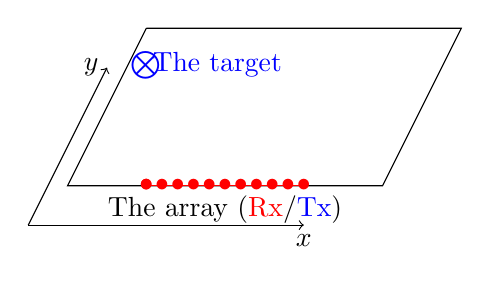
\begin{tikzpicture}
	\draw (0,0) -- (4,0)--(3,-2)--(-1,-2) -- (0,0);
	\draw [red](0,-2) -- (2,-2);
	\draw [red] (0,-2) node {$\bullet$};
	\draw [blue] (0,-0.4678) node {$\bigotimes$};
	\draw [blue] (0.9,-0.4678) node {The target};
	\foreach \x in {0,...,10}
	\draw [red] (0.2*\x,-2) node {$\bullet$};
	\draw (1,-2.3) node {The array (\textcolor{red}{Rx}/\textcolor{blue}{Tx})};
	\draw [->](-1.5,-2.5) -- (-0.5,-0.5);
	\draw [->](-1.5,-2.5) -- (2,-2.5);
	\draw (2,-2.7) node {$x$};
	\draw (-0.7,-0.5) node {$y$};
\end{tikzpicture}
	\end{frame}

\section{Pulse compression}
\begin{frame}
	\frametitle{Pulses}
\begin{itemize}
	\item \textbf{Waveforms}: LFM upchirp and downchirps
	\item We use both TDMA (upchirp only) and CDMA (both up and down chirps)
	\item Therefore, the two \textbf{waveforms should be orthogonal} (or at least, have a low cross-correlation)
\end{itemize}
\begin{columns}
	\begin{column}{0.5\textwidth}
		\begin{equation*}
			\begin{aligned}
				s_{TX, up}(t) &= \exp\left\{2j\pi\left(\left( f_c - B/2\right)t + \alpha t^2\right)\right\}\mathbb{1}_{0\leq t\leq T_p}(t)\\
				s_{TX, down}(t) &= \exp\left\{2j\pi\left(\left( f_c + B/2\right)t - \alpha t^2\right)\right\}\mathbb{1}_{0\leq t\leq T_p}(t)
			\end{aligned}
		\end{equation*}
	\end{column}
\begin{column}{0.5\textwidth}
\begin{table}
	\begin{tabular}{ccccc}
		\hline
		\hline
		Parameter& $f_c (\si{\kilo\hertz})$& $B (~\si{\kilo\hertz})$ & $f_s (\si{\kilo\hertz})$&$T_p (~\si{\milli\second})$ \\
		\hline
		Value&$10^3$&$10^3$&$2\times 10^2$&$10$\\
		\hline
	\end{tabular}
\end{table}
\end{column}
\end{columns}

\begin{columns}
	\begin{column}{0.5\textwidth}
		\begin{figure}[h!]
			\includegraphics[width=0.7\textwidth]{question1/lfm_up_stft}
			\centering
			\caption{LFM upchirp}
		\end{figure}
	\end{column}
\begin{column}{0.5\textwidth}
	\begin{figure}[h!]
		\includegraphics[width=0.7\textwidth]{question1/lfm_down_stft}
		\centering
		\caption{LFM downchirp}
	\end{figure}
\end{column}
\end{columns}
\begin{itemize}
	\item \textbf{STFT parameters} : zero padding $= \times 4$, $L = 512$ and $D = 32$  see \texttt{utils/fourier\_analysis.py}
\end{itemize}
\end{frame}

\begin{frame}
	\frametitle{Are the pulses truly orthogonal?}
\begin{columns}
	\begin{column}{0.5\textwidth}
		\begin{figure}[h!]
			\includegraphics[width=0.8\textwidth]{question1/cross_corr_plot}
			\centering
			\caption{Normalized cross-correlation}
		\end{figure}
	\end{column}
	\begin{column}{0.5\textwidth}
	\begin{itemize}
		\item The two pulses \textbf{are not} truly orthogonal...
		\item \textbf{Limited cross-talk}: $PCRR\approx 0.09\ll1$
		\item $PCRR\approx 0.09\approx\dfrac{1}{\sqrt{BT_p}}=\dfrac{1}{\sqrt{10^4\times 10^{-2}}} = 0.1$
		\item The chirps \textbf{can be considered as orthogonal}
		\item We can \textbf{separate} signals from the left and rightmost transmitters when working with the CDMA dataset
	\end{itemize}
	\end{column}
\end{columns}
Additional remarks:
\begin{itemize}
	\item The pulses are \textbf{over-sampled}: $f_s=2\times 10^{2}~\si{\kilo\hertz}\gg f_{max} = f_c + B/2 = 15~\si{\kilo\hertz}$
	\item Except if the reflectors frequency responses have components above $15~\si{\kilo\hertz}$
	\item Moreover, up-sampling the data can \textbf{considerably improve} the time-delay estimation (using pulse-compression)
	\item \textbf{Which normalization}? The same as in \texttt{MATLAB}: $C_{xy}\leftarrow C_{xy} / (\rVert x\lVert\cdot\rVert y\lVert)$
\end{itemize}
\end{frame}
\begin{frame}[fragile]
	\frametitle{Pulses}
\begin{lstlisting}[language=Python, style = mystyle, caption=LFM pulse generator]
def lfm_pulse(B: float, f_c: float,T_p: float, fs: float) -> np.array :

	'''This function computes and returns int(f_s*T_p) samples of a Linear Frequency Modulated (LFM).
	Note that if you want an UP LFM pulse, you need to use a positive bandwidth B. For a DOWN LFM pulse, 
	use a negative one.
	
	Inputs:
	- B: float, bandwidth in Hertz (Hz)
	- f_c: float, pulse central frequency in Hertz (Hz)
	- T_p: float, pulse length in seconds (s)
	- f_s: float, pulse sampling frequency in Hertz (Hz) 
	
	Output:
	- pulse: np.array (dtyp = 'complex'), LFM pulse'''

	'''First, we compute the chirp rate alpha (in 1/s^2) definded as the bandwidth divided by the pulse length
	alpha = B/T_p.'''
	alpha = B / T_p
	
	'''Then, we create a time np.array from t = 0 s to t = T_p with a time sampling interval of 1/fs which corresponds
	to a total number of points of int(Tp * fs).'''
	time = np.linspace(0, T_p, int(T_p * fs))
	
	'''We allocate space for the pulse array. Note that this array must be a complex array!'''
	pulse = np.zeros((int(T_p * fs) + 1), dtype= 'complex')
	
	'''Finally, we compute the pulse using the LFM pulse formula:
	 pulse[k] = exp(2j * pi * ( (fc - B / 2) * t + alpha * t ** 2 / 2) )'''
	pulse = np.exp(2 * 1j * np.pi * ((f_c - B/2) * time + alpha * time ** 2 / 2))
	
	'''We return the pulse array.'''
	
	return pulse
\end{lstlisting}
\end{frame}
\begin{frame}[fragile]
	\frametitle{Code}
\begin{itemize}
	\item Given an input pulse (\texttt{ping}, $x[k]$) and its echo (\texttt{echo}, $y[k]$), the output of the \textbf{match filter} (the compressed pulse) is given by:
	\begin{align*}
		z[n] = C_{yx}[n] = y \ast x[n]
	\end{align*}
	\item Note that we use the mode \texttt{'same'} inside \texttt{np.correlate}: the cross-correlation has the same size the output (or the maximum size of the inputs if they differ)
\end{itemize}
\begin{lstlisting}[language=Python, style = mystyle, caption=Pulse compression code]
	
def run_pulse_compression(ping : np.array, echo : np.array) -> np.array:

	'''This function returns a pulse compressed version of the input ping echo 
	using 'ping' as reference.
	
	Inputs:
	- ping: np.array (dtype = 'complex'), array of the transmitted signal
	- echo: np.array (dtype = 'complex'), array of the received echo
	
	Output:
	- pulse_compressed_signal: np.array (dtype = 'complex'), array of the pulse compressed singal'''
	
	'''We run the match filter in the time domain using numpy's correlate function.'''
	pulse_compressed_signal = np.correlate(echo, ping, mode = 'same')
	'''Normalization step: we normalize the cross-correlation by the product of the ping and the echo norms.'''
	pulse_compressed_signal /= (np.linalg.norm(ping) * np.linalg.norm(echo))
	
	'''We return the normalized cross-correlation'''
	
	return pulse_compressed_signal
	
\end{lstlisting}

\end{frame}

\begin{frame}
\frametitle{Pulse compression for TDMA data}
\begin{itemize}
	\item We apply pulse compression for the TDMA data $\implies$ the \textbf{reference signal} is the LFM UP chirp
\end{itemize}
\begin{columns}
\begin{column}{0.5\textwidth}
	\begin{figure}[h!]
		\includegraphics[width=0.8\textwidth]{question1/plot_after_before_pulse_compression_tdma_channel_4_1_upchirp.pdf}
		\centering
		\caption{Pulse compression, TDMA data, $N_{tx}=1$, $N_{rx}=4$}
	\end{figure}
\end{column}
\begin{column}{0.5\textwidth}
		\begin{figure}[h!]
		\includegraphics[width=0.8\textwidth]{question1/tdma_all_compressed_pulses_upchirp_1.pdf}
		\centering
		\caption{Pulse compression for $N_{tx}=1$, and all receivers, TDMA data}
	\end{figure}
\end{column}
\end{columns}
\begin{itemize}
	\item All the data / energy is \textbf{compressed} in the \textbf{shortest possible time extent}
	\item The match filter output is flat outside the peak (for CDMA data, this is not the case)
	\item When we run pulse compression for all the 32 receivers, we observe that the delay corresponding to the maximum increases: DOA or near-field (limit $d_{f}=\dfrac{D^2}{2\lambda}$)
\end{itemize}
\end{frame}

\begin{frame}
	\frametitle{Theoretical and practical time resolutions}
\begin{columns}
	\begin{column}{0.5\textwidth}
		\begin{itemize}
			\item The match filter acts as a cross-correlation between the chirp and its echo
			\item Assuming that both the reflector and the medium \textbf{dot not alter the waveform}, the echo is a delayed version of the chirp
			\item Therefore, there is only one time delay such that the echo perfectly overlaps the chirp 
			\item This explain why the output signal has a peak and is flat elsewhere
			\item All the data / energy is compressed in the shortest possible time extent. Both signals contain the same amount of data about the scene
			\item \textbf{What it the the shortest possible time extent? }
			\item \textbf{Theoretical time resolution:} $\delta t_{t} = \dfrac{1}{B}= 0.10~\si{\milli\second}$
			\item \textbf{Practical time-resolution:} $\delta t_{m} = 0.13~\si{\milli\second}$
			\item Perfectly symmetric $\mathrm{sinc}$ pattern
			\item Note that there is no AWGN here! 
		\end{itemize}
	\end{column}

\begin{column}{0.5\textwidth}
	\begin{figure}[h!]
	\includegraphics[width=0.8\textwidth]{question1/pulse_compressed_time_resolution_1_4.pdf}
	\centering
	\caption{Pulse compression resolution for $N_{tx}=1$$N_{rx}=4$, TDMA data}
\end{figure}
\end{column}
\end{columns}
\end{frame}
\section{Virtual array}
\begin{frame}
	\frametitle{Theoretical resolutions}
\begin{itemize}
	\item \textbf{Virtual array:} constructed by placing a virtual element at the between a Tx/Rx pairs for all possible pairs
\end{itemize}
\begin{columns}
	\begin{column}{0.33\textwidth}
		\begin{figure}[h!]
			\includegraphics[width=0.8\textwidth]{question2/rx_and_tx_postions.pdf}
			\centering
			\caption{Physical array}
		\end{figure}
	\end{column}
	\begin{column}{0.33\textwidth}
	\begin{figure}[h!]
		\includegraphics[width=0.8\textwidth]{question2/virtual_array_left_tx.pdf}
		\centering
		\caption{Virtual array (using only the leftmost transmitter and all receivers)}
	\end{figure}
\end{column}
	\begin{column}{0.33\textwidth}
	\begin{figure}[h!]
		\includegraphics[width=0.8\textwidth]{question2/virtual_array_all_tx.pdf}
		\centering
		\caption{Virtual array (using all receivers and transmitters)}
	\end{figure}
\end{column}
\end{columns}
\begin{itemize}
	\item When using two transmitters instead of one, we double the number of virtual elements ($N=N_{tx}N_{rx}$)
	\item Is the virtual 'well built'? The element spacing $d$ \textbf{should be less or equal} to $\lambda/2$ to avoid \textbf{aliasing}
	\item Lowest wavelength: $\lambda = \dfrac{c}{f_c + B/2} = 22.7~\si{\milli\meter}$ and $\lambda/2=11.3~\si{\milli\meter}$
	\item \textbf{With only one Tx and all receivers:} $d=17.0~\si{\milli\meter}>\dfrac{\lambda}{2}$ \textcolor{red}{\faTimes}
	\item \textbf{With all Tx and all Rx:} $d=8.5~\si{\milli\meter}<\dfrac{\lambda}{2}$ \textcolor{green}{\faCheck}
\end{itemize}
\end{frame}
\begin{frame}
\frametitle{Theoretical resolutions}
\begin{itemize}
\item \textbf{Lateral resolution} (in rad): $\delta\beta = \dfrac{\lambda}{2L_{SA}}$
\item Which frequency? We use the minimum frequency $f_{min}=B+\frac{f_c}{2}=15~\si{\kilo\hertz}\leftrightarrow 22.7~\si{\milli\meter}$ to obtain \textbf{the best achievable resolution}
\item $\delta\beta = \dfrac{22.7\times 10^{-3}}{2\times 1.054}=1.08\times 10^{-2}~\si{\radian}$
\item \textbf{Along-track} resolution at a range of $R=4~\si{\meter}$: $\delta x = R\delta\beta=4\times 1.08\times 10^{-2} = 43.1~\si{\milli\meter}$
\item \textbf{Cross-track} resolution: $\delta y=\dfrac{c}{2B}=\dfrac{340}{2\times 10\times 10^{3}}= 17~\si{\milli\meter}$
\end{itemize}
\end{frame}
\section{Delay-And-Sum}
\begin{frame}[fragile]
\frametitle{DAS algorithm}
\begin{itemize}
	\item The presented algorithm is a simplified version of the one I used
	\item Please see \texttt{utils/parallel\_DAS\_beamforming.py} for the code used to generate the following images
	\item This code uses parallel computing which significantly improve the computation time of the image!
\end{itemize}
\begin{lstlisting}[language=Python, style = mystyle, caption=Pulse compression code]
def DAS_imaging_TDMA(grid_config : dict, rx_positions : np.array, tx_positions : np.array, tdma_data : np.array, B : float, fc : float,c : float, T_p : float, N_t : float, fs : float) -> np.array:

	x_values = np.arange(grid_config['x_min'],  grid_config['x_max'], grid_config['x_step'])
	n_x = len(x_values)
	y_values = np.arange(grid_config['y_min'],  grid_config['y_max'], grid_config['y_step'])
	n_y = len(y_values)
	image = np.zeros((n_x, n_y), dtype = 'complex')
	up_pulse = lfm_pulse(B = B, f_c = fc, T_p = T_p, fs = fs)
	N_rx = len(rx_positions)
	N_tx = len(tx_positions)
	for n_rx in tqdm(range(N_rx)):
		for n_tx in range(N_tx):
			echo = tdma_data[:, n_rx, n_tx]
			compressed_pulse = run_pulse_compression(ping = up_pulse, echo = echo)
			tmp_image = np.zeros_like(image, dtype = 'complex')
			tx_pos = tx_positions[n_tx]
			rx_pos = rx_positions[n_rx]
			for j in range(n_x):
				for k in range(n_y):
					pixel_x_pos = x_values[j]
					pixel_y_pos = y_values[k]
					tx_to_pixel_distance = np.sqrt((pixel_x_pos - tx_pos) ** 2 + pixel_y_pos ** 2)
					rx_to_pixel_distance = np.sqrt((pixel_x_pos - rx_pos) ** 2 + pixel_y_pos ** 2)
					time_delay = (tx_to_pixel_distance + rx_to_pixel_distance) / c
					if index_delay < N_t:
						tmp_image[j, k] += compressed_pulse[index_delay]
			image += tmp_image
return x_values, y_values, image.T
\end{lstlisting}
\end{frame}

\begin{frame}
	\frametitle{Experimental setup}
\begin{itemize}
	\item To image the scene, we use the following grid:
	\begin{itemize}
		\item $x$-axis: $[-5,5]~\si{\meter}$ with a resolution of $10~\si{\milli\meter}$ ($10^{3}$ points)
		\item $y$-axis: $[0,5]~\si{\meter}$ with a resolution of $5~\si{\milli\meter}$ ($10^{3}$ points)
	\end{itemize} 
\item Impossible to know if the target lies between $0$ and $5~\si{\meter}$ or $0$ and $-5~\si{\meter}$ because of the array symmetry along the $x$-axis
\item Given the pulse compressed time series, we expect to find only one reflectors, in the upper left part of the image
\item Thereby, we assume that the target is located between $0$ and $5~\si{\meter}$
\item Since the is no noise, the point scatterer will be clearly distinguishable from the background (no energy)
\end{itemize}
\begin{columns}
	\begin{column}{0.5\textwidth}
		\begin{figure}[h!]
			\includegraphics[width=0.8\textwidth]{question3/TDMA_DAS_image.pdf}
			\centering
			\caption{TDMA dataset, all Tx/Rx}
		\end{figure}
	\end{column}
	\begin{column}{0.5\textwidth}
		\begin{figure}[h!]
			\includegraphics[width=0.8\textwidth]{question3/TDMA_DAS_image_with_noise.pdf}
			\centering
			\caption{TDMA dataset,  all Tx/Rx + noise}
		\end{figure}
	\end{column}
\end{columns}
\end{frame}
\begin{frame}
	\frametitle{DAS on TDMA dataset}

\begin{columns}
	\begin{column}{0.5\textwidth}
		\begin{figure}[h!]
			\includegraphics[width=0.8\textwidth]{question3/TDMA_DAS_image.pdf}
			\centering
			\caption{TDMA dataset, all Tx/Rx}
		\end{figure}
	\end{column}
	\begin{column}{0.5\textwidth}
		\begin{figure}[h!]
			\includegraphics[width=0.8\textwidth]{question3/TDMA_DAS_image_one_transmit_0_0.pdf}
			\centering
			\caption{TDMA dataset, one transmit sequence (Tx $0\rightarrow~\text{Rx}~0$)}
		\end{figure}
	\end{column}
\end{columns}
\begin{itemize}
	\item Reflector position: $(x,y)=$. 
	\item The image shows the superposition of the pulse compresses delayed series. So, the brighter a pixel is, the better is the position estimate
	\item Note that the energy is spread in the reflector direction
	\item With one transmit: we have one arc-circle with maximum brightness. Since we use only one Rx/Tx couple, all the pixel which such that $r_r + r_t = d$ while have the same delay. This leads to the arc-circle pattern
\end{itemize}
\end{frame}

\begin{frame}
	\frametitle{Resolution}
\begin{tabular}{ccc}
	\hline
	Resolution (in $\si{\milli\meter}$)&Theoretical&Measured\\
	\hline
	\hline
	Along-track&43.1&47.0  \\
	Cross-track&17.0&25.5\\
	\hline
\end{tabular}
\end{frame}

\begin{frame}
	\frametitle{DAS on CDMA dataset}
How to deal with CDMA data?
\begin{itemize}
	\item We don't know which transmitter is used for the transmit sequences $\longleftrightarrow$ we don't if the used waveform is an up or downchirp
	\item Since the two waveforms are orthogonal, the pulse compression step will return a peak if we use the correct chirp and 0 if not (\textcolor{blue}{upchirp in the example})
	\item Using the linearity of the cross-correlation, we can modify the pulse compression step in the following way:
\begin{equation}
	C_{echo,chirps}(\tau) = C_{echo,upchirp + downchirp}(\tau) = \underbrace{C_{echo,upchirp}(\tau)}_{\textcolor{blue}{\approx 1}} + \underbrace{C_{echo,downchirp}(\tau)}_{\textcolor{blue}{\approx PCRR \approx 0.09}}
\end{equation}
\end{itemize}
\begin{columns}
	\begin{column}{0.5\textwidth}
		\begin{figure}[h!]
			\includegraphics[width=0.8\textwidth]{question3/TDMA_DAS_image.pdf}
			\centering
			\caption{TDMA dataset}
		\end{figure}
	\end{column}
	\begin{column}{0.5\textwidth}
		\begin{figure}[h!]
			\includegraphics[width=0.8\textwidth]{question3/CDMA_DAS_image.pdf}
			\centering
			\caption{CDMA dataset}
		\end{figure}
	\end{column}
\end{columns}
\end{frame}

\begin{frame}
	\frametitle{DAS on CDMA dataset}
\begin{columns}
	\begin{column}{0.5\textwidth}
		\begin{figure}[h!]
			\includegraphics[width=0.8\textwidth]{question3/TDMA_DAS_image.pdf}
			\centering
			\caption{TDMA dataset}
		\end{figure}
	\end{column}
	\begin{column}{0.5\textwidth}
		\begin{figure}[h!]
			\includegraphics[width=0.8\textwidth]{question3/CDMA_DAS_image.pdf}
			\centering
			\caption{CDMA dataset}
		\end{figure}
	\end{column}
\end{columns}
\begin{itemize}
	\item Using CDMA data leads to the same position estimate
	\item Nevertheless, one can notice the circle pattern is wider than for TDMA dataset
	\item This side lobe is caused by the fact that the waveforms are not truly orthogonal
	\item Moreover, the is a wide side lobe at $(3,3)~\si{\meter}$
	\item Pollution level
	\item Resolution
\end{itemize}
\end{frame}

\section{Tapering}
\begin{frame}

\end{frame}

		
	
\end{document}